The normalisation of the $Z$+hf background is estimated 
from data as included as freely floating parameter in 
the final fit. This normalisation is mainly determined 
from the dedicated $Z$+HF dilepton control region.

Relative acceptance uncertainties are applied on $Z$+hf
in the other regions included in the fit, 
the \hadhad signal region and the \lephad 
signal regions, to take into account potential differences 
in the normalisation between the CR and the SRs.
 
In each signal region also shape variations are checked 
and applied, correlated with the relative acceptance uncertainties on the normalisations, where they are found to be relevant as described in the following. 

All these uncertainties are derived by MC-to-MC comparison, 
as described in Section~\ref{sec:systematics_backgroundmodelling}, 
following the \href{https://twiki.cern.ch/twiki/bin/viewauth/AtlasProtected/PmgWeakBosonProcesses}{\underline{recommendations of the PMG group for Weak Boson processes}}. 


Only Z + heavy flavour jets background are considered, 
including $Z$+bb, $Z$+bc, $Z$+cc. 
Contributions from Z + light flavour jets 
such as $Z$+l, $Z$+bl and $Z$+cl are excluded. 

Uncertainties due to choice of generators are evaluated
by comparing the Sherpa 2.2.1 samples to the
Madgraph+Pythia8 samples. 
Uncertainties on the $Z$+jets background modelling 
related to the choice of renormalisation and factorisation 
scales are evaluated using event weights included 
in the Sherpa 2.2.1 samples, varying the scales either together 
or independently up and down by a factor of two, 
leading to 7-point scale variations. 
The scale uncertainty is then given by the maximum shift 
of the envelope with respect to the nominal, from which 
the envelope around the nominal can be worked out. 
The uncertainty due to the choice of PDF set is evaluated 
in a similar way, using the event weights included in the samples. 
The PDF variations include 100 replicas of the nominal NNPDF3.0 PDF set 
as well as central values for two different PDF set, 
MMHT2014nnlo68cl and CT14nnlo, and two NNPDF3.0nnlo $\alpha_s$ variations.  
The NNPDF intra-PDF uncertainty is estimated as the standard deviation 
of the set of 101 NNPDF3.0 sets. 
The envelope of the differences between the nominal NNPDF set 
and the other two PDF sets is taken as an additional uncertainty. 

From the nominal Sherpa configuration there are two other parameters 
that can be varied to investigate uncertainties 
on the modelling of the $W$/$Z$+jets process: 
Matrix element matching (ckkw), which varies the scale taken 
for the calculation for the overlap between jets 
from the matrix element and the parton shower. 
The nominal value for this parameter is 20 GeV. 
The up variation increases this to 30 GeV, 
while the down variation decreases the nominal value to 15 GeV. 
The second parameter is the resummation scale (qsf), 
which varies the scale used for the resummation 
of soft gluon emission $\mu_{qsf}$ is varied from 2 and with respect to the nominal. 

Relative acceptance normalisation uncertainties between the CR and the SRs are calculated 
from the single channel acceptances using Equation~\ref{eq:relative_acceptance_unc} 
and are found in the different fit regions to be 
as large as reported in Table~\ref{sec:systs:tab:systematics_normalisations_ZHF}.


\begin{table}
\centering
\small
\begin{tabular}{|c|c|c|c|}
\hline
Source & Size in LepHad SLT & Size in LepHad LTT & Size in HadHad\\
\hline
ME & +0.021, -0.021 & +0.10, -0.10 & -0.07, +0.07\\
Scales & -0.029, +0.053 & -0.054, +0.085 & -0.096, +0.12\\
CKKW & +0.07, -0.07 &  +0.071, -0.071 & +0.053, -0.053\\
QSF & -0.016, +0.016 & -0.016 , +0.016 & +0.06, -0.06 \\
PDF+$\alpha_s$ & -0.0026, +0.0026 & -0.0033 , +0.0033 & -0.0077, +0.0077 \\
PDF choice & -0.0097, +0.0097 & -0.011, +0.011 & -0.0098, +0.0098\\
Total & -0.081, +0.092 & -0.14, +0.15 & -0.14, +0.16\\
\hline
\end{tabular}
\caption{Relative size of relative acceptance normalisation uncertainties on $Z$+HF for the di-Higgs analysis.}
\label{sec:systs:tab:systematics_normalisations_ZHF}
\end{table}


\paragraph{Uncertainties on $Z$+HF in the \lephad channel}\mbox{}\\

In the $\tau_{lep}\tau_{had}$ channel the parametrizations of the shape uncertainties 
are derived separately for the SLT channel and the LTT channel. 
Only shape is considered and hence all samples are scaled to one.

The Madgraph samples for comparison are with DSID 361510-361514 for
$m_{ll} > 40$~GeV and 361638-361642 for $10$~GeV $< m_{ll} < 40$~GeV, 
sliced in number of partons. The shape discrepancy between the nominal Sherpa 
samples and the Madgraph samples are propagated through the PNN 
output score. In most of the bins and mass points 
no significant deviation is observed within statistical uncertainty, 
as shown in Appendix~\ref{subsec:appendix_systs_ZHFsysts_lephad}. 
Therefore this uncertainty is ignored for the \lephad channel. 
Furthermore, various kinematic variables are tested to parametrise
the difference in the PNN score where no variables have a significant impact. 


%Uncertainties on the $Z$+jets background modelling related to the choice of renormalisation and factorisation scales are evaluated using event weights included in the Sherpa 2.2.1 samples, varying the scales either together or independently up and down by a factor of two, leading to 7-point scale variations. The scale uncertainty is then given by the maximum shift of the envelope with respect to the nominal, from which the envelope around the nominal can be worked out.
For the scale variations the envelope is characterised 
by the $p_T$ of the two $b$-jets, $p_T^{BB}$, 
as shown in Fig.\ref{fig:lephad_ZHF_scale_pTBB} for the SLT channel the LTT channel. 
Only the shape variation is considered. The discrepancy between 
the nominal sample and the variation sample 
is propagated through the PNN output score, 
the results are shown in Appendix~\ref{subsec:appendix_systs_ZHFsysts_lephad}.

%The uncertainty due to the choice of PDF set is evaluated in a similar way, using the event weights included in the samples. The PDF variations include 100 replicas of the nominal NNPDF3.0 PDF set as well as central values for two different PDF set, MMHT2014nnlo68cl and CT14nnlo, and two NNPDF3.0nnlo $\alpha_s$ variations.  The NNPDF intra-PDF uncertainty is estimated as the standard deviation of the set of 101 NNPDF3.0 sets. The envelope of the differences between the nominal NNPDF set and the other two PDF sets is taken as an additional uncertainty. 

For the PDF variations no obvious shape dependence 
is observed in the PNN score distribution 
comparing the nominal NNPDF set and the standard deviation 
of the 100 replicas. Similarly, no obvious shape dependence 
is found for neither the additional uncertainty CT14nnlo and MMHT2014nnlo68cl 
nor the $\alpha_s$ variations. 
The PNN score distributions of these uncertainties variation 
are shown in Appendix~\ref{subsec:appendix_systs_ZHFsysts_lephad}. 

%From the nominal Sherpa configuration there are another two parameters that can be varied to investigate uncertainties on the modelling of the $W$/$Z$+jets process: Matrix element matching (ckkw), which varies the scale taken for the calculation for the overlap between jets from the matrix element and the parton shower. The nominal value for this parameter is 20GeV. The up variation increases this to 30GeV, whilst the down variation decreases the nominal value to 15GeV. The second parameter is the resummation scale (qsf), which varies the scale used for the resummation of soft gluon emission $\mu_{qsf}$ is varied from 2 and with respect to the nominal. 
The up and down variation for the CKKW and QSF 
uncertainties are both smaller than the nominal sample yields, 
and the solution for this issue is to normalize 
the central value of the up and down variation to the nominal sample, 
and take the difference from there. 
After symmetrizing no shape dependence is observed. 
The PNN score distributions is shown in Appendix~\ref{subsec:appendix_systs_ZHFsysts_lephad}.


\begin{figure}[!h]
\centering
\subfloat[]{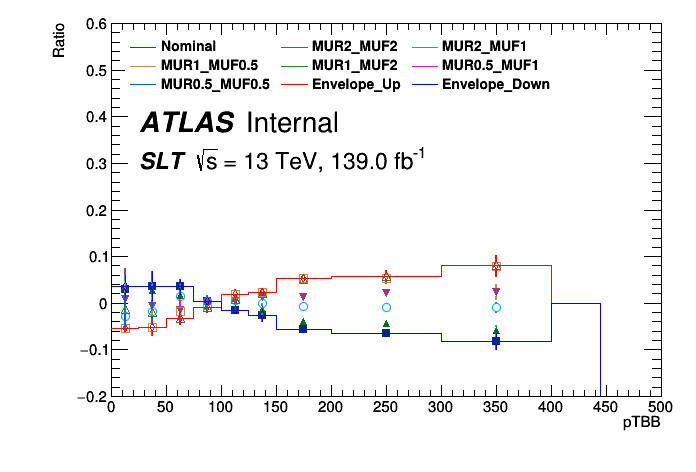
\includegraphics[width=.41\textwidth]{figures/lephad_modelling_systs/SLT/ZHF_scale/Ratio_pTBB_Norm.png}}\quad
\subfloat[]{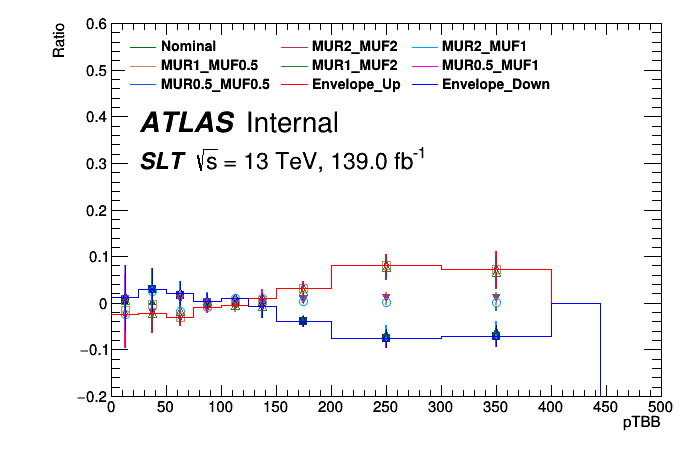
\includegraphics[width=.41\textwidth]{figures/lephad_modelling_systs/LTT/ZHF_scale/Ratio_pTBB_Norm.png}}\quad
\caption{SLT (left) and LTT channel (right): Taking an envelope of the $Z$+HF scale variation with $p_T$ of the 2 $b$-jets.}
\label{fig:lephad_ZHF_scale_pTBB}
\end{figure}


\paragraph{Uncertainties on $Z$+HF in the \hadhad channel}\mbox{}\\

The shape dependence of scales variations are described by the shape of the envelope of 7-point variation, which is directly derived by the maximun (for 1up variation) and minimum (for 1down variation) bin-by-bin on the BDT/PNN score distributions, as shown in Fig.~\ref{fig:hadhad_ZHF_Scale_SMBDT}. Although the \texttt{muR\_muF} may give the largest shape variation for most of the MVA scores, it is shown that the envelope can also estimate the shape dependence reasonably well. Figures for more MVA distributions and detailed studies can be found in Appendix~\ref{subsec:appendix_systs_ZHFsysts_hadhad} and \href{https://indico.cern.ch/event/1042450/contributions/4422123/attachments/2269878/3854717/Z%2Bjets%20modelling%20v3.pdf}{\underline{those slides}}

The comparison with Madgraph samples introduces an shape uncertainty in the $\tau_{had}\tau_{had}$ channel. 
The shape variation can be approximately described by a linear function of the mass of b-jet system ($m_{BB}$), as shown in Fig.~\ref{fig:hadhad_ZHF_Madgraph_mBB}. In $m_{BB}>250$~GeV, the variation is considered to be the same as that at 250 GeV.
Due to the limited statistic of the Madgraph samples, it is still possible that the shape dependence that we observed is originated from fluctuations. 

More details can be found in Appendix~\ref{subsec:appendix_systs_ZHFsysts_hadhad}.

\begin{figure}[htbp]
    \centering
    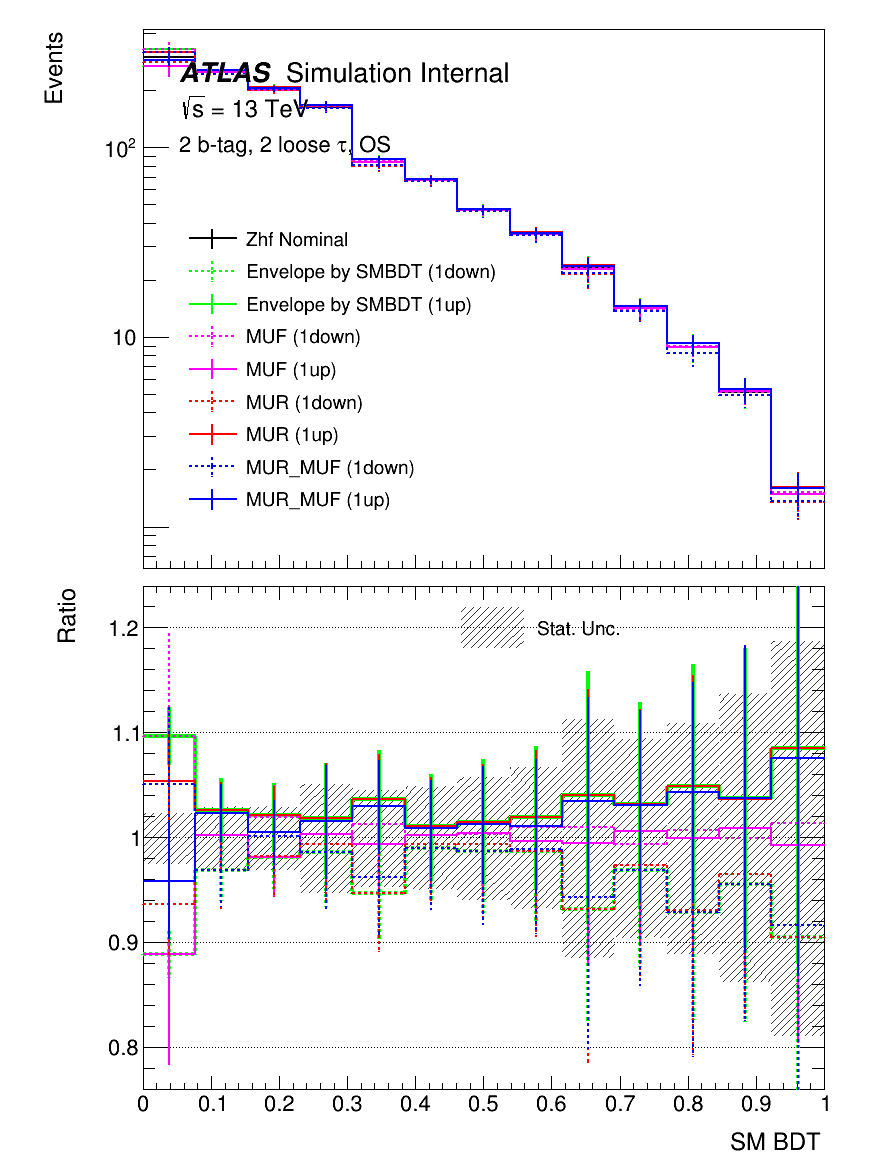
\includegraphics[width=.45\textwidth]{figures/systs/hadhad_ZHF/2tag2pjet_0ptv_LL_OS_SMBDT_BDT_Scale.png}
    \caption{Shape uncertainty of scale ($\mu_R$, $\mu_F$) variations on SMBDT. The black(nominal), pink, red and blue histograms/ratios are the 7-point variations, while the green one is the envelope. Up/down variations are shown in solid/dashed lines. The SMBDT score is transformed into the binning of the final fit. The shaded area shows the statistical uncertainty of the nominal samples.}
    \label{fig:hadhad_ZHF_Scale_SMBDT}
\end{figure}

\begin{figure}[htbp]
    \centering
    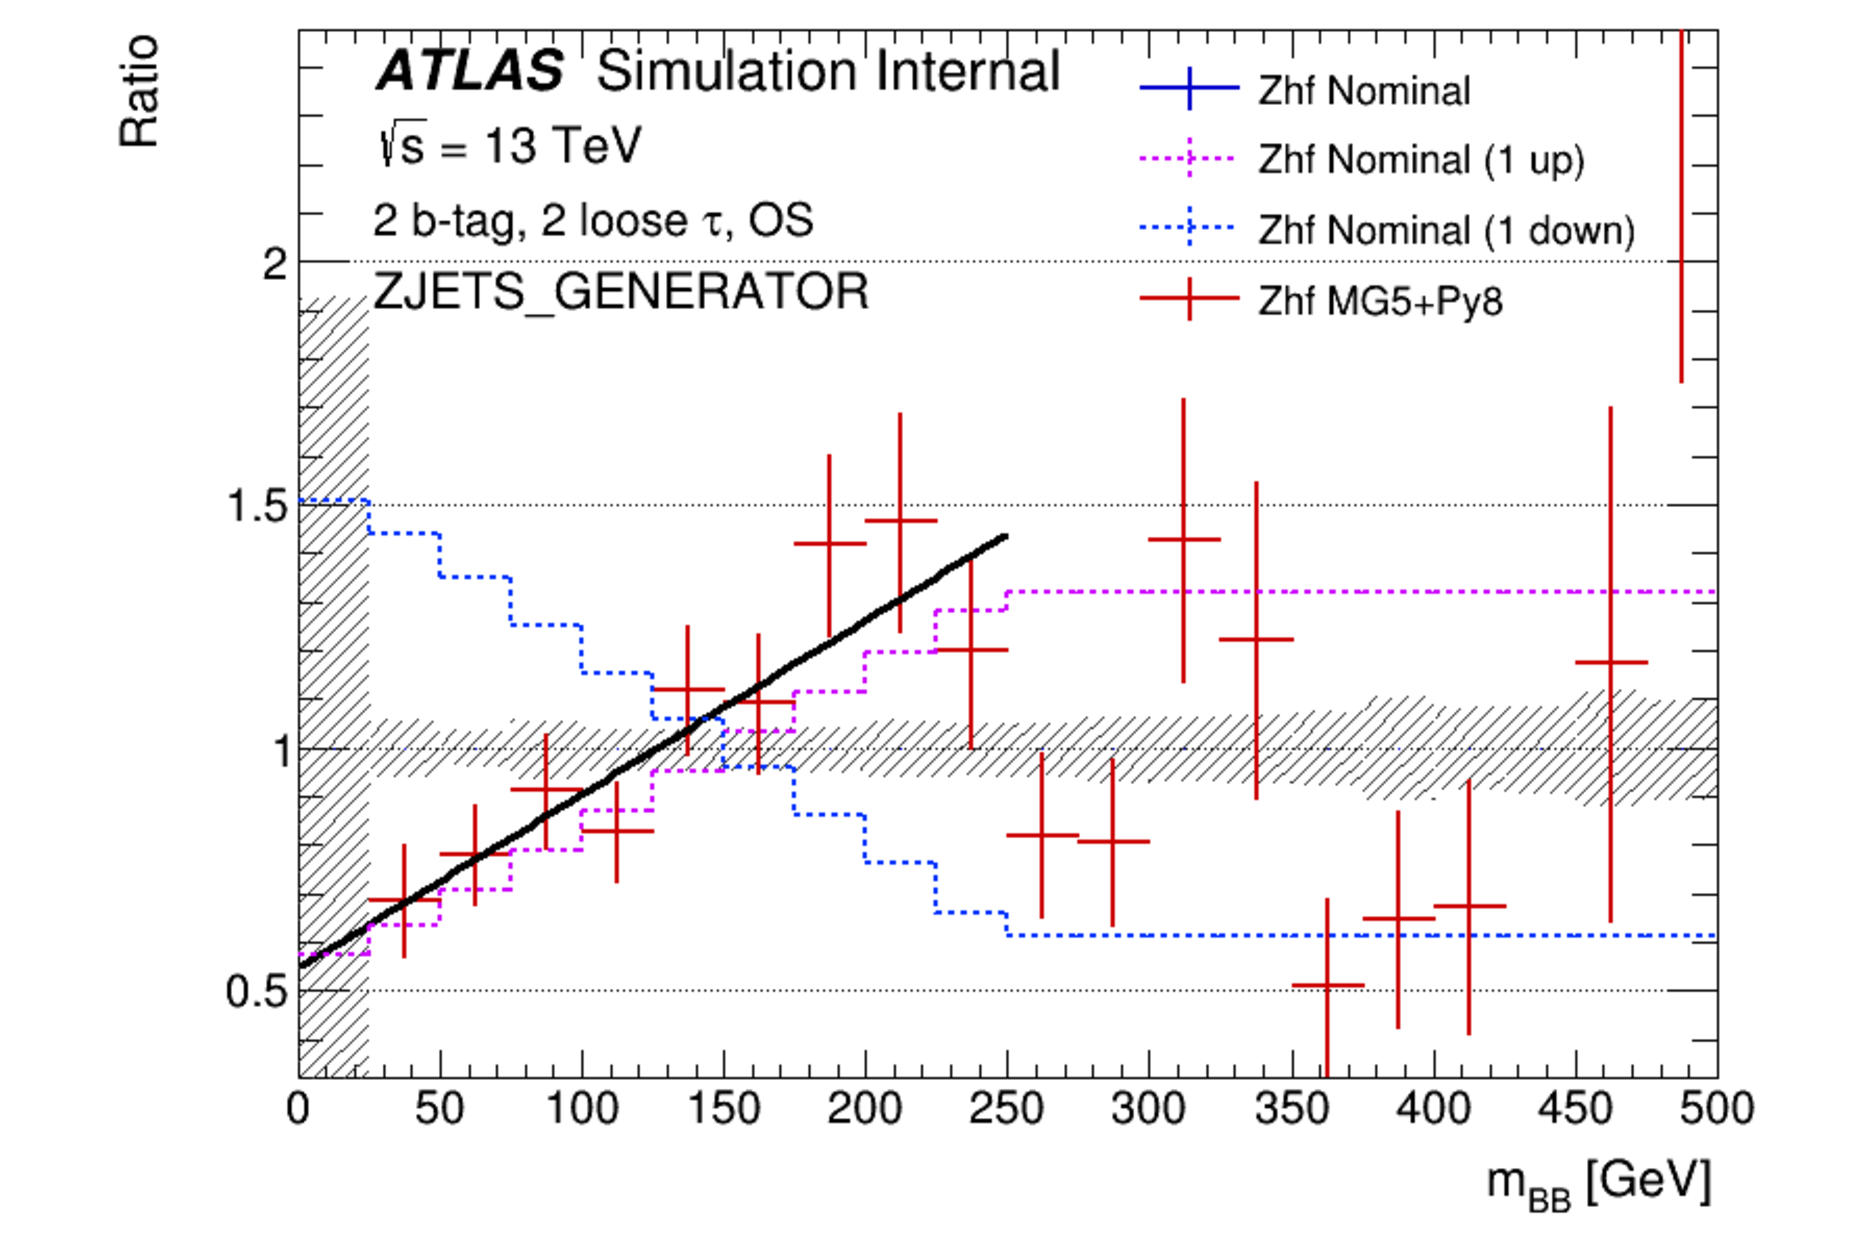
\includegraphics[width=.45\textwidth]{figures/systs/hadhad_ZHF/2tag2pjet_0ptv_LL_OS_mBB_Presel}
    \caption{Madgraph comparison uncertainty of Z+HF in the HH $\tau_{had}\tau_{had}$ signal region. The "Nominal" samples are generated by Sherpa, "MG5+Py8" represents the Madgraph samples. The black line in the ratio plot is the parametrisation derived with the $m_{BB}$ distribution, which corresponds to the "up" variation~($0.55 + 0.0035 \times m_{BB}~\text{if}~m_{BB}\le 250~\GeV;~1.43~\text{if}~m_{BB} > 250~\GeV$). The down variation is the symmetric mirror of the up variation. The dotted lines are the final up and down variations estimated by the parametrised uncertainty. The shaded area shows the statistical uncertainty of the nominal samples.}
    \label{fig:hadhad_ZHF_Madgraph_mBB}
\end{figure}

Other shape uncertainties on the $Z$+HF background are neglected in the \hadhad signal region as they are found to be negligible, as shown in Appendix~\ref{subsec:appendix_systs_ZHFsysts_hadhad}.


\paragraph{Uncertainties on $Z$+HF background in the Z+HF control region}\mbox{}\\

Shape uncertainties on the $Z$+HF background are neglected in the Z+HF control region as they are found to be negligible in the $m_{ll}$ distribution included in the fit for this region, as shown in Appendix~\ref{subsec:appendix_systs_ZHFsysts_ZCR}.

